\documentclass{article}
\usepackage[serbian]{babel}
\usepackage{cmsrb}
\usepackage[OT2,T1]{fontenc}
\usepackage{hyperref}
\usepackage{amsmath}
\usepackage{graphicx}
\usepackage{hyperref}
\hypersetup{
    colorlinks,
    citecolor=black,
    filecolor=black,
    linkcolor=blue,
    urlcolor=blue
}

\begin{document}

\fontencoding{OT2}\selectfont

\title{{\huge Fazi klasterovanje}}

\author{Maja Crnomarkovi\'{c} 21/2017\\Marko Babi\'{c} 77/2017}
\date{25. jun 2021.}

\maketitle

\centerline{{\normalsize Seminarski rad u okviru kursa}}
\centerline{{\normalsize Ra\v{c}unarska inteligencija}}

\begin{figure}[h]
\vspace{1cm}
\centerline{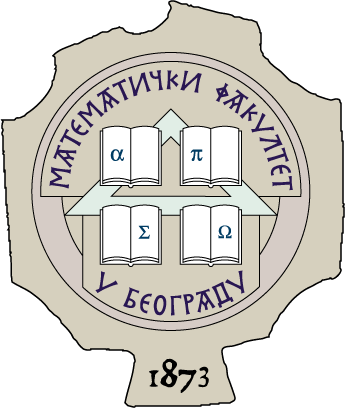
\includegraphics[scale=0.5]{images/grb.png}}
\end{figure}

\newpage

\renewcommand*\contentsname{\fontencoding{OT2}\selectfont Sadr\v{z}aj}

\tableofcontents

\newpage

\section{\fontencoding{OT2}\selectfont Uvod}
\textbf Segmentacija slika je jedan od najprostranjenijih na\v{c}ina za korektno klasifikovanje piksela u aplikacijama zasnovanim na odlu\v{c}ivanju. Segmentacija je tehnika koja particioni\v{s}e sliku na uniformne i nepreklapaju\'{c}e delove, zasnovano na nekoj meri sli\v{c}nosti. Ova tehnika ima veliki broj primena u analizi slika, medicinskom procesiranju slika, geografskom informacionom sistemu, i dr. Poslednjih godina, iskazano je veliko interesovanje za analizu slika, i s vremenom se ova oblast sve vi\v{s}e razvija. Na\v{s} rad se bavi problemom segmentacije slika kori\v{s}\'{c}enjem tehnike fazi klasterovanja. Najvi\v{s}e pa\v{z}nje \'{c}e biti posve\'{c}eno problemu detekcije tumora na mozgu segmentovanjem rendgenskih snimaka.


\subsection{\fontencoding{OT2}\selectfont Definicija klasterovanja}

Ne postoji formalna definicija klasterovanja. Klaster analiza je pronala\v{z}enje grupa objekata takvih da su objekti u jednoj grupi me\dj usobno sli\v{c}niji u odnosu na objekte u razli\v{c}itim grupama. \textbf{Klasterovanje} se odnosi na postupak izdvajanja klastera. Problem klasterovanja se mo\v{z}e definisati na slede\'{c}i na\v{c}in: Dat je \v{z}eljeni broj klastera $K$, skup podataka od $N$ ta\v{c}aka i funkcija za merenje rastojanja. Potrebno je prona\'ci particije skupa podataka tako da se minimizuje vrednost funkcije za merenje.

\subsection{\fontencoding{OT2}\selectfont Vrste klasterovanja}


\begin{itemize}

\item \textbf{Particiono klasterovanje}: Podela skupa podataka u nepreklapaju\'{c}e podskupove (klastere) takve da je svaki podatak ta\v{c}no u jednom podskupu.\\
\begin{figure}[h]
\fontencoding{OT2}\selectfont
\centerline{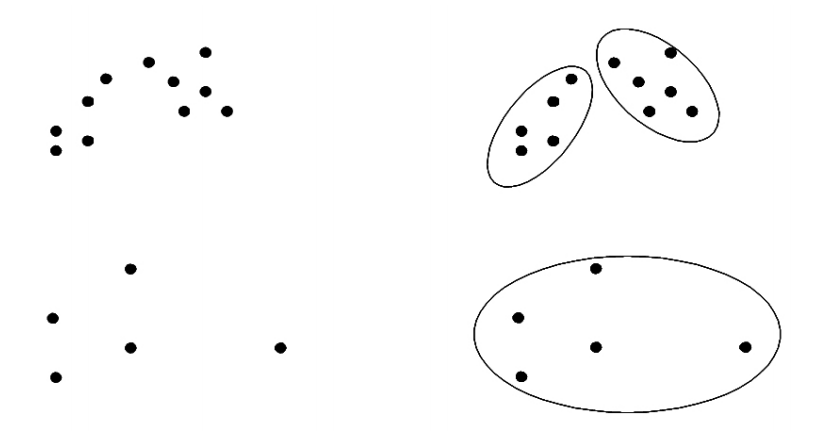
\includegraphics[scale=0.35]{images/part_klast.png}}
\caption{Levo - po\v{c}etni podaci. Desno - Particiono klasterovanje.}
\end{figure}
\item \textbf{Hijerarhijsko klasterovanje}: Skup ugnje\v{z}denih klastera organizovan u obliku hijerarhijskog stabla.
\begin{figure}[h]
\fontencoding{OT2}\selectfont
\centerline{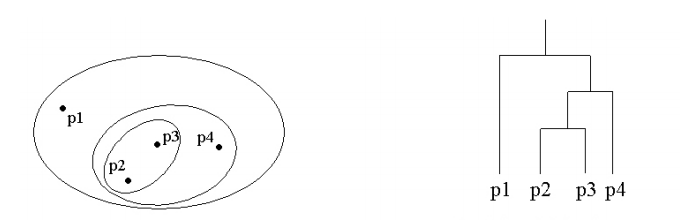
\includegraphics[scale=0.45]{images/hie_clast.png}}
\caption{Levo - hijerarhijsko klasterovanje. Desno - dengogram.}
\end{figure}

\end{itemize}

\subsection{\fontencoding{OT2}\selectfont Razli\v{c}iti tipovi klasterovanja}

\begin{itemize}
\item Ekskluzivno/neekskluzivno klasterovanje
\item Fazi (rasplinuto/nerasplinuto) klasterovanje
\item Delimi\v{c}no/komplentno klasterovanje
\item Heterogeno/homogeno klasterovanje
\end{itemize}

\subsection{\fontencoding{OT2}\selectfont Fazi klasterovanje}

Kod klasi\v{c}nog klasterovanja, podaci su podeljeni u odre\dj en broj disjunktnih klastera, gde jedan element mo\v{z}e pripadati samo jednom klasteru. U fazi klasterovanju ta\v{c}ka mo\v{z}e pripadati ve\'{c}em broju klastera sa nekom te\v{z}inom izme\dj u nula i jedan. Zbir svih te\v{z}ina je jednak 1. Sli\v{c}ne karakteristike ima verovatnosno klasterovanje. Fazi klasterovanje se jo\v{s} naziva i rasplinuto klasterovanje.


\section{\fontencoding{OT2}\selectfont Segmentacija slika}

Postoje mnogobrojne metode i raznovrsna literatura za izdvajanje informacija sa slike i njenu podelu na razli\v{c}ite regione. Svaka od tih metoda susre\'{c}e se sa odre\dj enim ograni\v{c}enjima koja se ogledaju u vremenskoj slo\v{z}enosti ili ta\v{c}nosti. Razlog za to je \v{s}to ne postoje jasne granice izme\dj u objekata na slici. Fazi klasterovanje pokazalo se kao veoma dobar na\v{c}in za prevazila\v{z}enje ovog problema.

Segmentacija slika kori\v{s}\'{c}enjem fazi klasterovanja bila je predmet velikog interesovanja kroz godine. Neki od algoritama koji se bave ovom temom su: Fazi c-sredina, Gustafon-Kese, Gausova razgradnja sme\v{s}e, Fazi c-sorte, Fazi c-prstenovi,  Prilagodljive fazi c-sorte, Fazi c-omota\v{c}i, Fazi c-sferni omota\v{c}i,  Fazi c-pravougaoni omota\v{c}i (eng. {\fontencoding{T1}\selectfont Fuzzy C-Means (FCM), Gustafson-Kesse (GK), Gaussian Mixture Decomposition (GMD), Fuzzy C-Varieties (FCV), Adaptive Fuzzy C-varieties (AFC), Fuzzy C-Shell (FCS), Fuzzy C-Spherical Shells (FCSS), Fuzzy C-Rings, Fuzzy C-Quadric Shells (FCQS), Fuzzy C- Rectangular Shells (FCRS)} i drugi. Me\dj u svim gore navedenim algoritmima, metod fazi c-sredina je najprihva\'{c}eniji na\v{c}in za segmentaciju slika jer omogu\'{c}ava manji gubitak informacija u odnosu na algoritme klasi\v{c}nog klasterovanja.

U nastavku \'{c}emo prikazati segmentaciju slika kori\v{s}\'{c}enjem algoritama k-sredina (eng. {\fontencoding{T1}\selectfont k-means}) i fazi c-sredina (eng. {\fontencoding{T1}\selectfont fuzzy c-means}).

\subsection{\fontencoding{OT2}\selectfont Fazi c-sredina}

Prvi put ga je predstavio Dun a potom ga je modifikovao Bezdek. Fazi c-sredina algoritam je iterativni algoritam koji poku\v{s}ava podeliti skup podataka u unapred zadat broj podgrupa(klastera) s tim \v{s}to ovde svaki element pripada svakom klasteru sa odre\dj enim stepenom pripadnosti koji je izme\dj u nula i jedan.

Sledi detaljan opis algoritma:

\begin{itemize}

\item Ulazni parametri: Podaci koje \v{z}elimo da klasterujemo (skup elemenata $x$ dimenizje $n$) i broj koji ozna\v{c}ava koliko klastera \v{z}elimo da dobijemo ($k$).
\item Izlazni paramteri: Matrica pripadnosti klasterima (dimenzije $n \times k$ ) i matrica centroida klastera(dimenzije $k \times d$ gde je $d$ dimenzija svakog pojedina\v{c}nog elementa iz skupa $x$).

\end{itemize}

Koraci algoritma:

\begin{enumerate}

\item Nasumi\v{c}no dodeljujemo vrednosti za sve te\v{z}ine u oznaci: $w_{ij}, \\ 1\leq i \leq n, \quad 1\leq i \leq n$ uz uslove:
\begin{enumerate}
\item $ \sum_{j=1}^k w_{ij} = 1, \quad \forall i\in {1,2,...,n}$
\item $ 0 < \sum_{i=1}^n w_{ij} < n, \quad \forall j\in {1,2,...,k} $
\end{enumerate}
\item Ra\v{c}unanje centroida za sve klastere u oznaci $c_j$ pomo\'{c}u formule:
\begin{equation}
c_j = \frac{\sum_{i=1}^n w_{ij}^p x_i}{\sum_{i=1}^n w_{ij}^p}
\end{equation}
Napomena: ako je $p = 0$, ima\'{c}emo pona\v{s}anje klasi\v{c}nog k-sredina algoritma.
\item A\v{z}uriranje vrednosti matrice pripadnosti koriste\'{c}i formulu:
\begin{equation}
w_{ij} = \frac{\frac{1}{dist(x_i, c_j)}^\frac{1}{p-1}}{\sum_{q=1}^k \frac{1}{dist(x_i, c_q)}^\frac{1}{p-1}}
\end{equation}
\item Ponavljati korake 2. i 3. dok centroidi ne ostanu isti u dve iteracije za redom.

\end{enumerate}

Mera kvaliteta klasterovanja je suma kvadratne gre\v{s}ke(eng. {\fontencoding{T1}\selectfont Sum of Squared Error}):
\begin{equation}
SSE = \sum_{j=1}^k\sum_{i=1}^n w_{ij}^p dist(x_i, c_j), \quad p \in 1,...,\infty
\end{equation}

\subsubsection{\fontencoding{OT2}\selectfont Na\v{s}a implementacija algoritma fazi c-sredina}

Re\v{s}enje problema segmentacije slika uz pomo\'{c} algoritma fazi c-sredina smo implementirali u programskom jeziku Pajton. 
Pajton biblioteke kori\v{s}\'{c}ene u na\v{s}em re\v{s}enju su:
\begin{itemize}
\item $numpy$
\item $matplotlib.pyplot$
\item $os$
\item $cv2$
\item $time$
\item $math$
\end{itemize}
Algoritam je implementiran u funkciji $fuzzy\_c\_means()$. Ona kao argumente prima:
\begin{itemize}
\item $data$ - niz podataka(to je ustvari matrica koja je dimenzije $n \times d$);
\item $n$ - ceo broj koji ozna\v{c}ava broj podataka koje \v{z}elimo da klasterujemo;
\item $k$ - ceo broj koji ozna\v{c}ava broj klastera;
\item $d$ - ceo broj koji ozna\v{c}ava dimenziju pojedina\v{c}nog podatka iz skupa podataka koje \v{z}elimo da klasterujemo;
\item $p$ - ceo broj koji ozna\v{c}ava paramear za fazi formulu kojom odre\dj ujemo stepen pripadnosti nekog podatka za svaki od klastera;
\item $max\_iter$ - ceo broj koji ozna\v{c}ava maksimalni broj iteracija zbog bezbednosti,
\end{itemize}
dok kao povratnu vrednost vra\'{c}a:
\begin{itemize} 
\item matricu $n \times k$ u kojoj \'{c}e element na poziciji biti $w_{ij}$, tj. te\v{z}ina sa kojom {\fontencoding{T1}\selectfont i}-ti element pripada {\fontencoding{T1}\selectfont j}-tom klasteru;
\item matricu $k \times d$ u kojoj \'{c}e se \v{c}uvati centroidi svih klastera.
\end{itemize}
Dakle, kako je jedna slika predstavljena kao matrica piksela gde je svaki piksel dimenzije tri, nju parsiramo u niz, kori\v{s}\'{c}enjem funkcije  $ reshape() $ iz Pajton biblioteke $ numpy $, kako bismo je mogli, kao argument, proslediti na\v{s}oj funkciji. Nakon \v{s}to na\v{s}a funkcija kao povratnu vrednost vrati matricu pripadnosti podataka(u na\v{s}em slu\v{c}aju piksela dimenzije tri) klasterima, svakom od piksela dodeljujemo vrednost centroida klastera za koji je vrednost najve\'ca u matrici pripadnosti. Zatim niz piksela vra\'{c}amo u matricu polaznih dimenzija kori\v{s}\'{c}enjem funkcije  $ reshape() $ i posmatramo je kao sliku.\\

\fontencoding{OT2}\selectfont

\newpage

\subsubsection{\fontencoding{OT2}\selectfont Rezultati algoritma fazi c-sredina}

Nakon opisanog postupka slike ispisujemo kori\v{s}\'{c}enjem funkcija $ subplot() $ i $ imshow() $ iz Pajton biblioteke $ cv2 $.\\
Slike koje je segmentovao na\v{s} algoritam fazi c-sredina izgledaju ovako:

\begin{figure}[h!]
\centerline{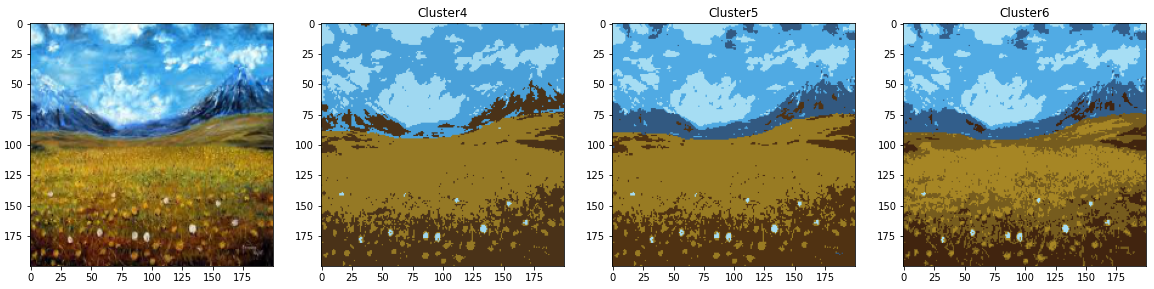
\includegraphics[scale=0.45]{images/segmented_fuzzy_c_means1.png}}
\centerline{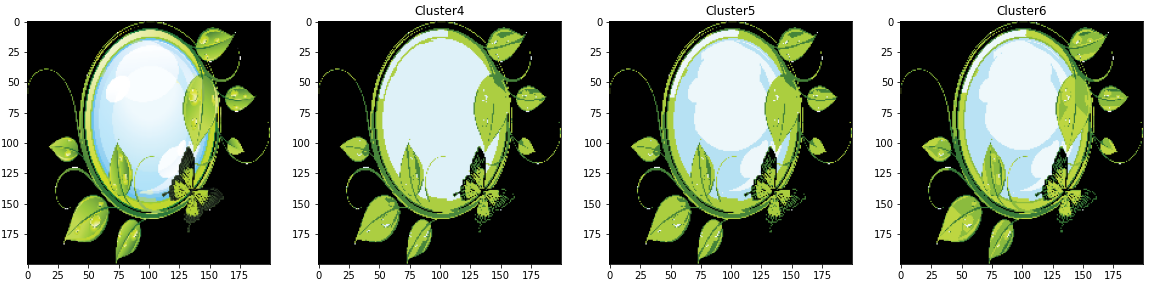
\includegraphics[scale=0.45]{images/segmented_fuzzy_c_means3.png}}
\centerline{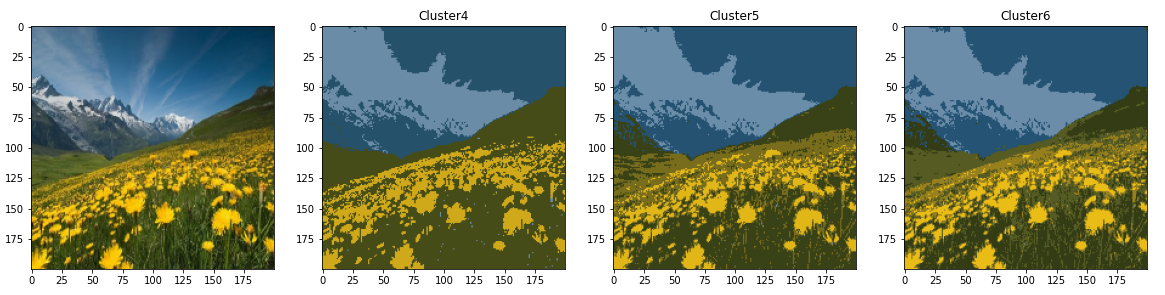
\includegraphics[scale=0.45]{images/segmented_fuzzy_c_means6.png}}
\end{figure}

\newpage

\begin{figure}[h!]
\centerline{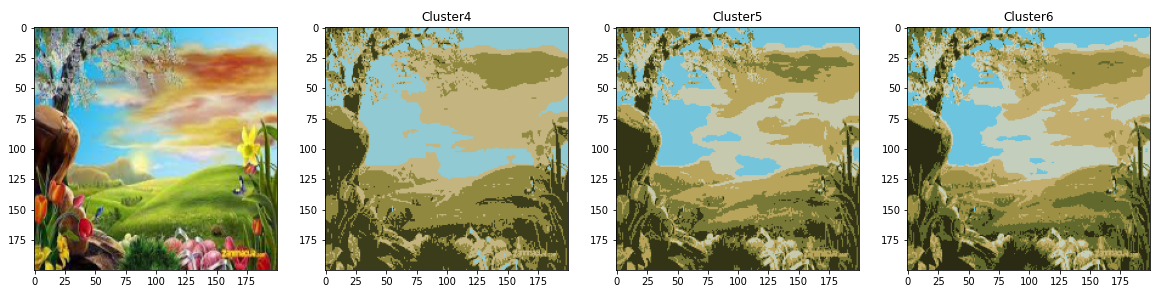
\includegraphics[scale=0.45]{images/segmented_fuzzy_c_means7.png}}
\centerline{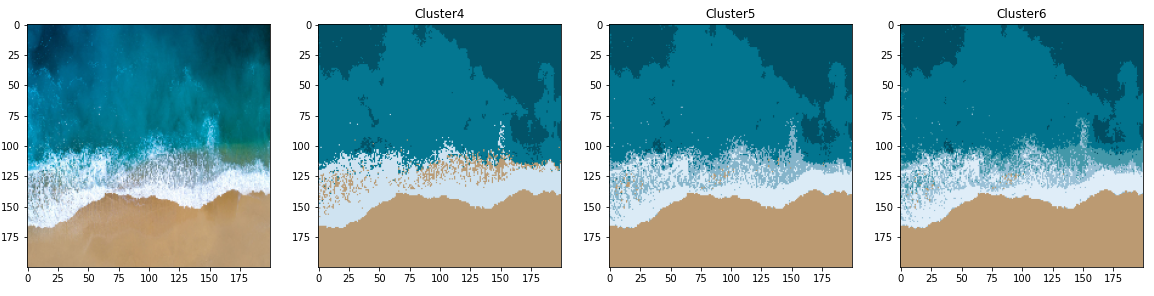
\includegraphics[scale=0.45]{images/segmented_fuzzy_c_means8.png}}
\centerline{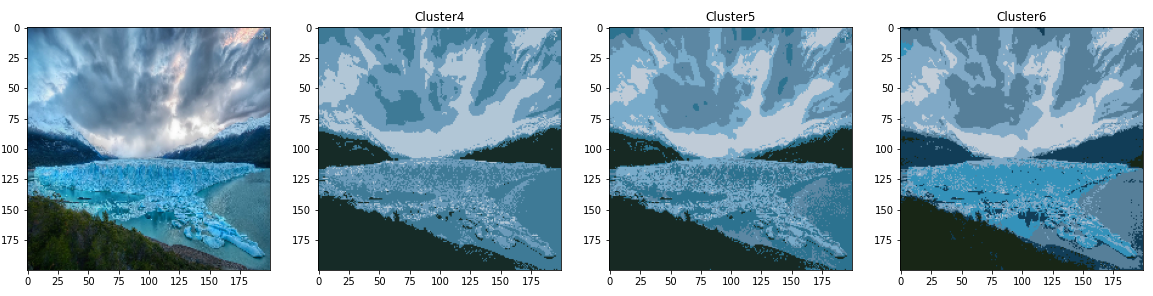
\includegraphics[scale=0.45]{images/segmented_fuzzy_c_means5.png}}
\centerline{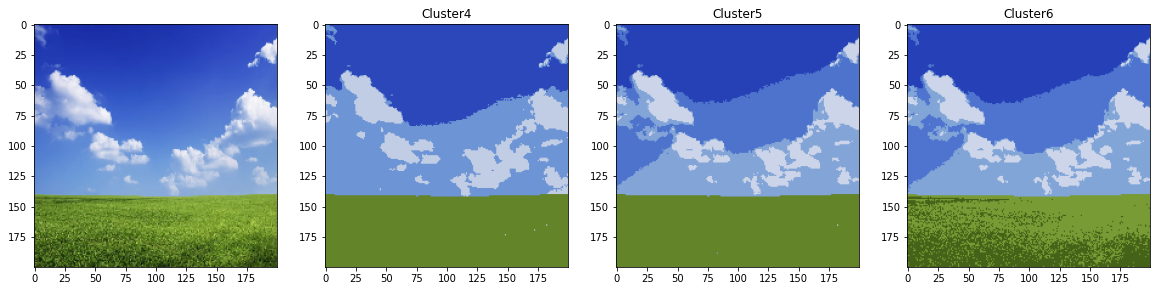
\includegraphics[scale=0.45]{images/segmented_fuzzy_c_means4.png}}
\end{figure}

\newpage

\begin{figure}[h!]
\centerline{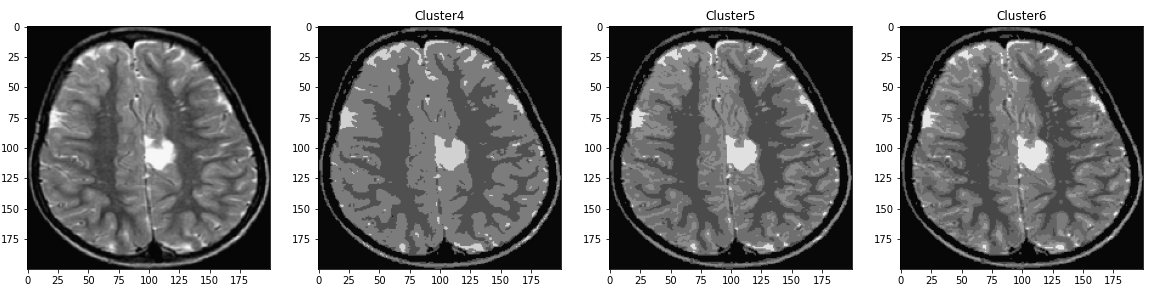
\includegraphics[scale=0.45]{images/segmented_fuzzy_c_means9.png}}
\centerline{ 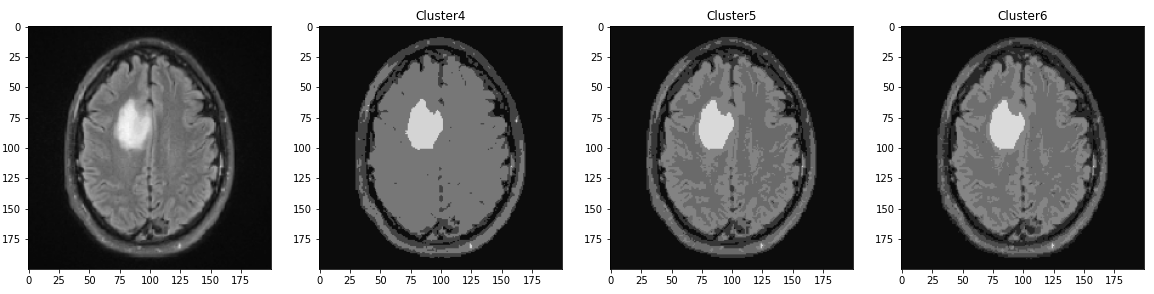
\includegraphics[scale=0.45]{images/segmented_fuzzy_c_means11.png}}
\centerline{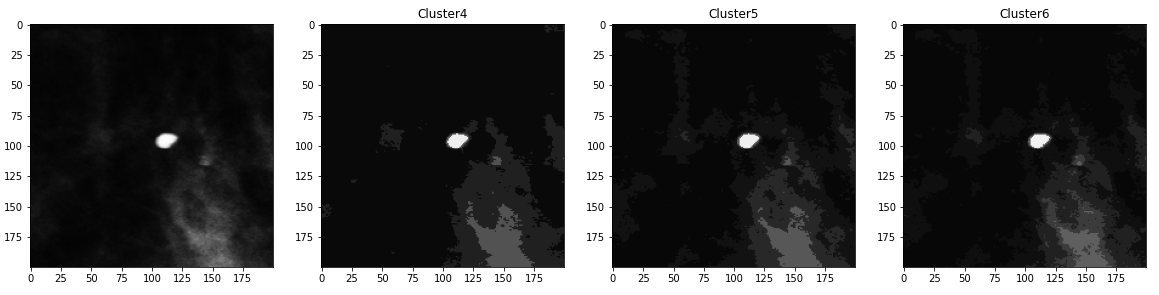
\includegraphics[scale=0.45]{images/segmented_fuzzy_c_means12.png}}
\centerline{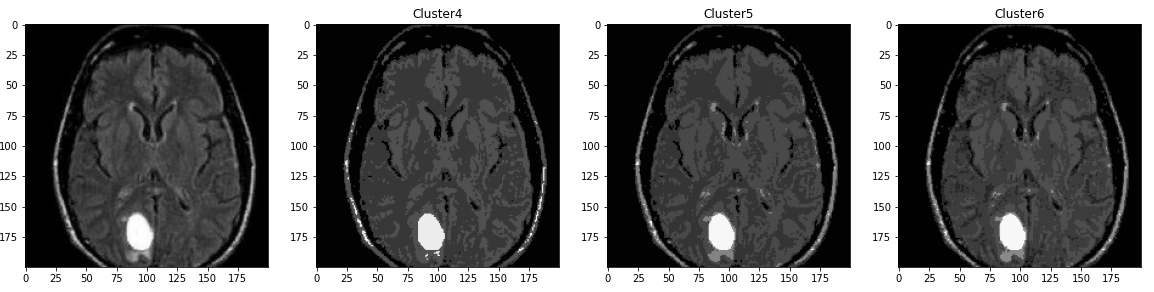
\includegraphics[scale=0.45]{images/segmented_fuzzy_c_means13.png}}
\end{figure}

\newpage

\begin{figure}[h!]
\centerline{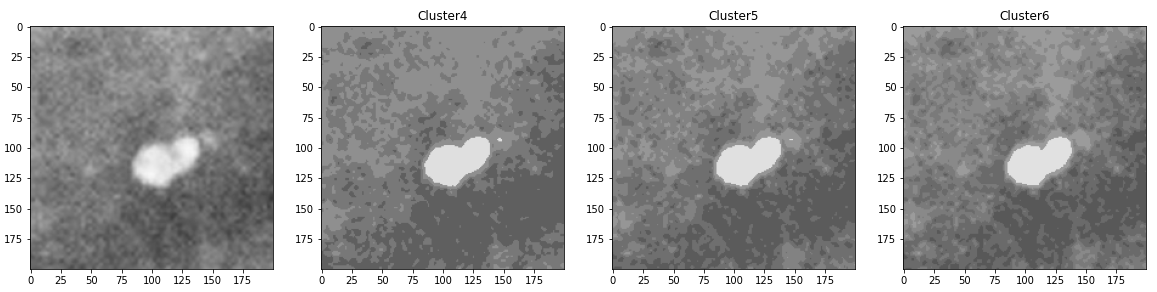
\includegraphics[scale=0.45]{images/segmented_fuzzy_c_means0.png}}
\centerline{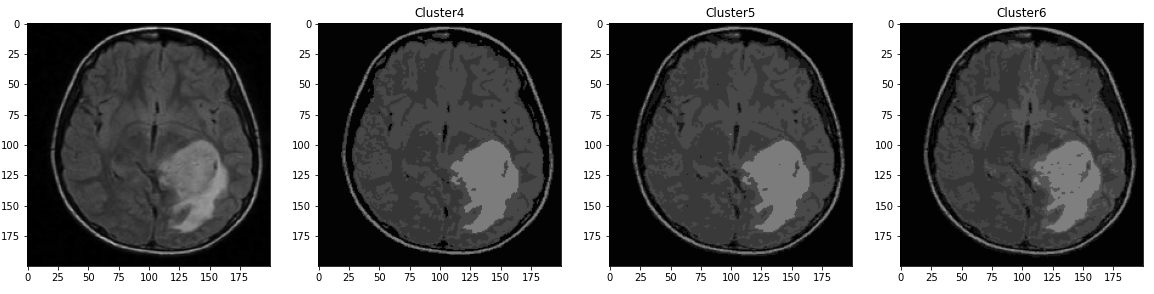
\includegraphics[scale=0.45]{images/segmented_fuzzy_c_means10.png}}
\centerline{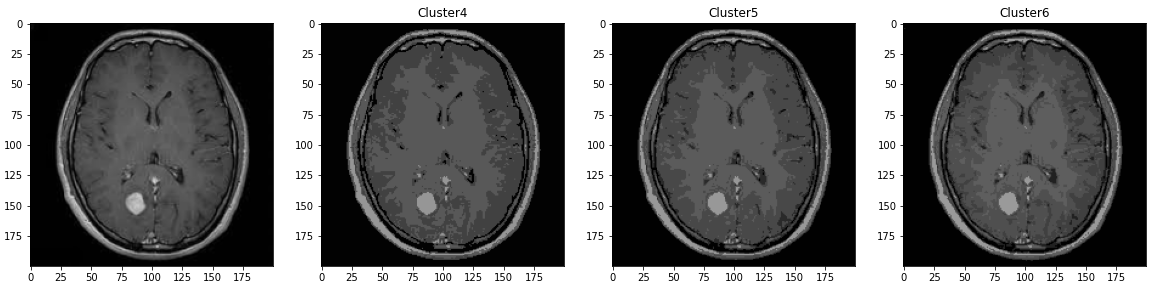
\includegraphics[scale=0.45]{images/segmented_fuzzy_c_means2.png}}
\end{figure}

Kori\v{s}\'{c}enje vi\v{s}e klastera:

\newpage

\begin{figure}[h!]
\centerline{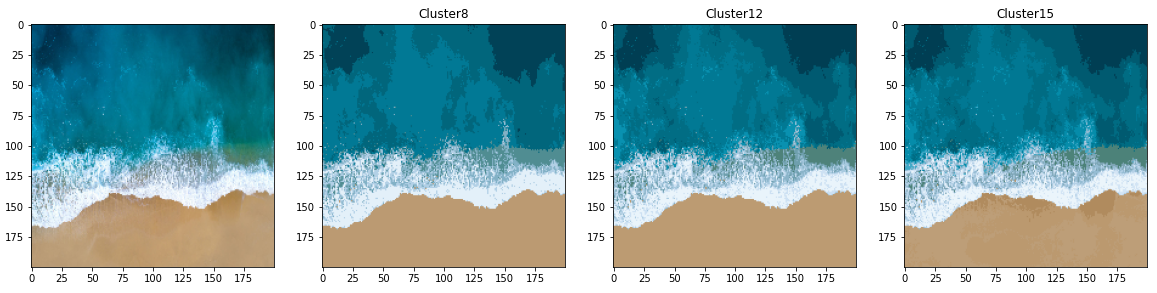
\includegraphics[scale=0.45]{images/ultra_segmented_fuzzy_c_means0.png}}
\centerline{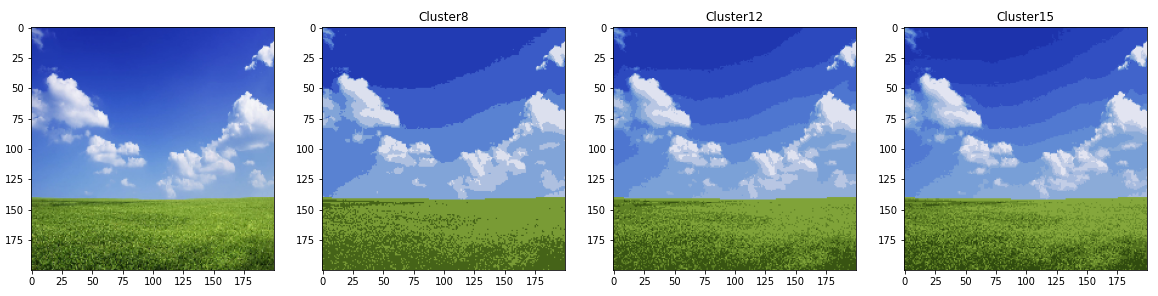
\includegraphics[scale=0.45]{images/ultra_segmented_fuzzy_c_means1.png}}
\centerline{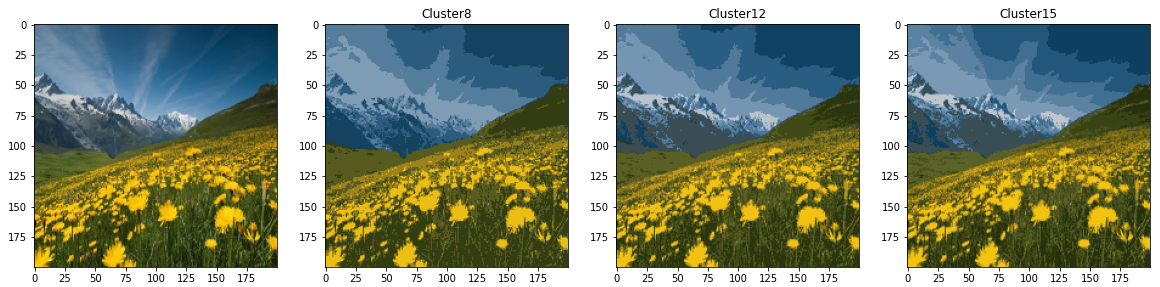
\includegraphics[scale=0.45]{images/ultra_segmented_fuzzy_c_means2.png}}
\end{figure}

Kori\v{s}\'{c}enje manje klastera:

\newpage

\begin{figure}[h!]
\centerline{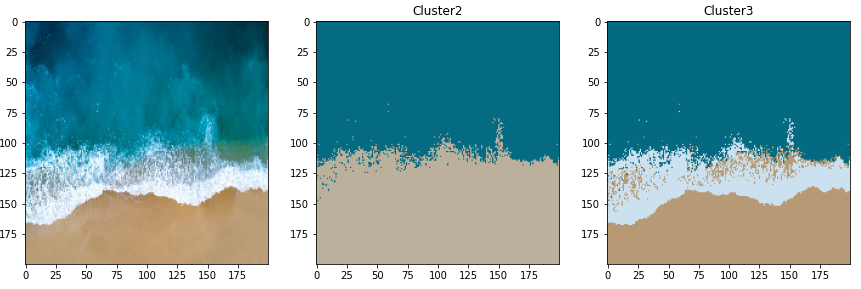
\includegraphics[scale=0.45]{images/low_segmented_fuzzy_c_means0.png}}
\centerline{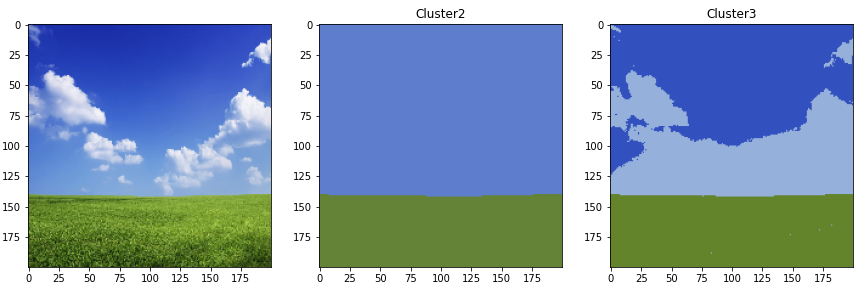
\includegraphics[scale=0.45]{images/low_segmented_fuzzy_c_means1.png}}
\centerline{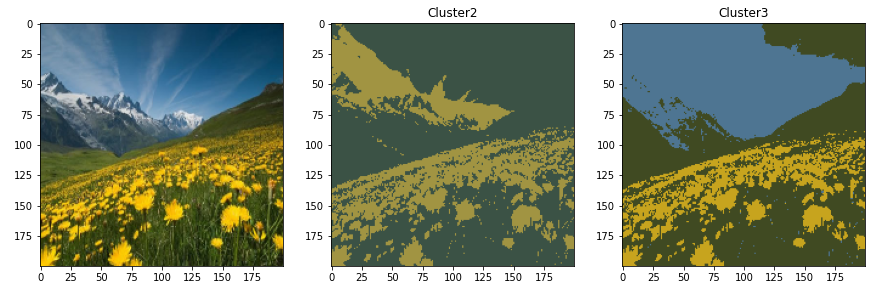
\includegraphics[scale=0.45]{images/low_segmented_fuzzy_c_means2.png}}
\end{figure}

U slu\v{c}aju rendgenskih snimaka mozga vrlo je bitno da se jasno segmentuje odre\dj eni detalj na slici, odnosno tumor ako on postoji, i zbog toga nakon gore opisanog postupka binarizujemo sliku kori\v{s}\'{c}enjem funkcije $ threshold() $ iz biblioteke $ cv2 $ i piksele predstavljamo jednom celobrojnom vredno\v{s}\'{c}u, odnosno predstavljamo sliku sa samo dve boje. Ovaj postupak je detaljno opisan u odeljku \ref{text:threshold}.\\


Nakon primene na\v{s}eg algoritma fazi c-sredina, funkcije $ threshold() $ i parsiranja slike u matricu piksela koji su dimenzije jedan na rendgenske snimke tumora mozga na izlazu dobijamo slike segmentovane na slede\'{c}i na\v{c}in:

\newpage

\begin{figure}[h!]
\centerline{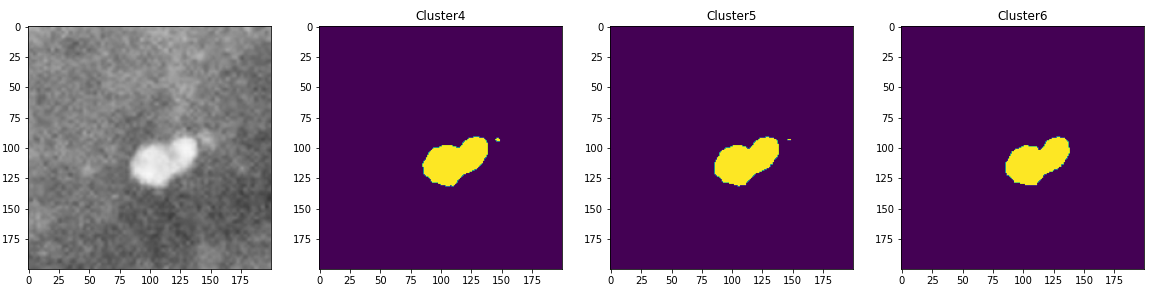
\includegraphics[scale=0.45]{images/segmented_fuzzy_c_means_tumor0.png}}
\centerline{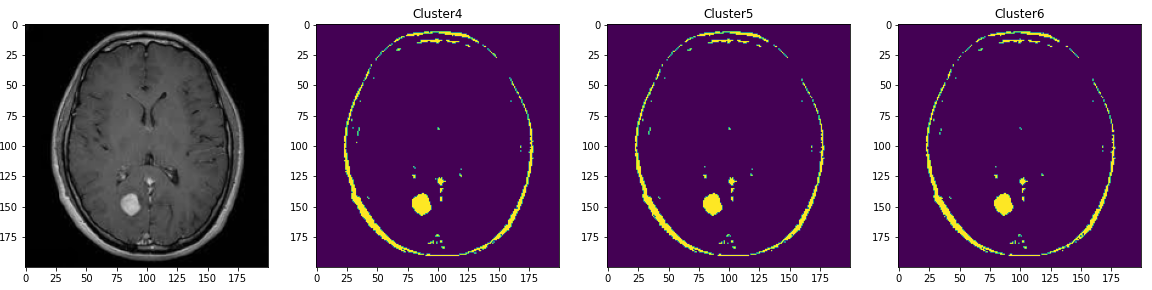
\includegraphics[scale=0.45]{images/segmented_fuzzy_c_means_tumor1.png}}
\centerline{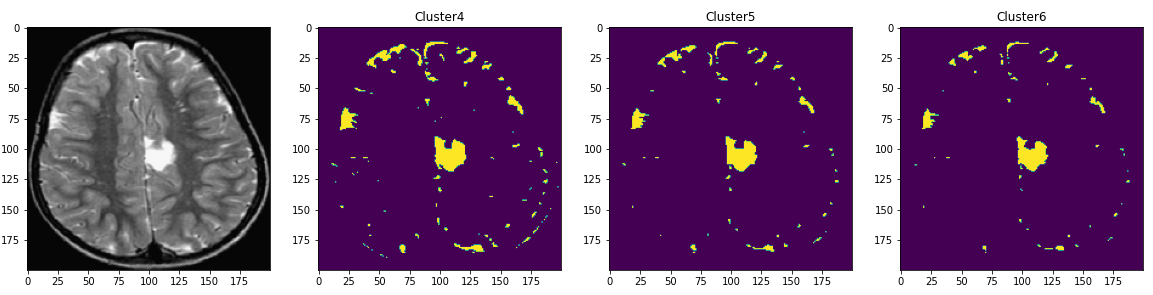
\includegraphics[scale=0.45]{images/segmented_fuzzy_c_means_tumor2.png}}
\centerline{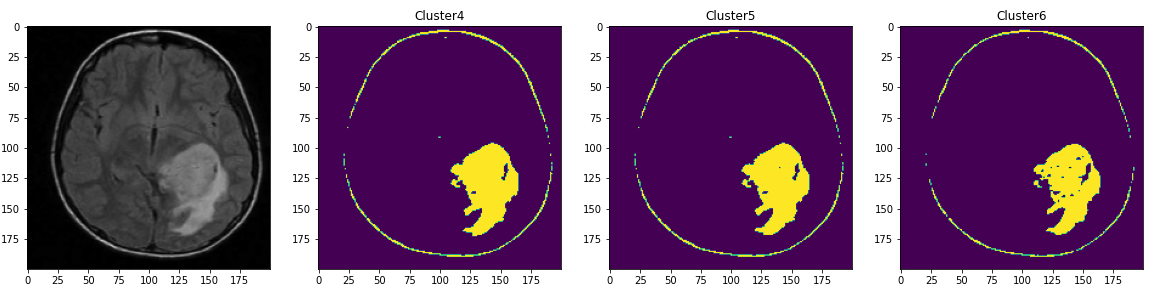
\includegraphics[scale=0.45]{images/segmented_fuzzy_c_means_tumor3.png}}
\end{figure}

\newpage

\begin{figure}[h!]
\centerline{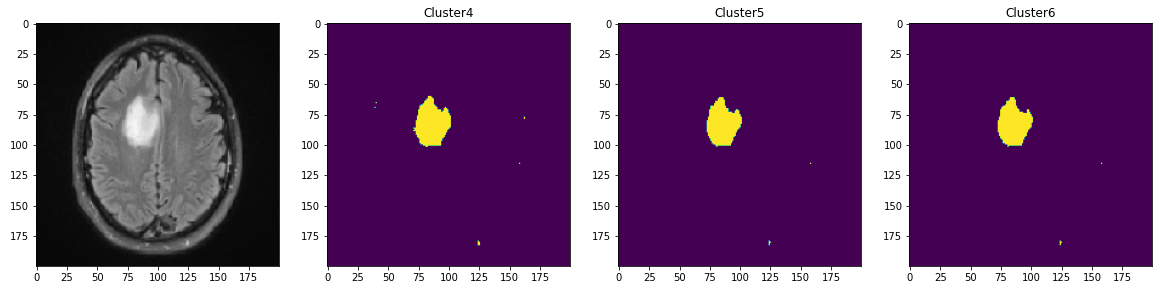
\includegraphics[scale=0.45]{images/segmented_fuzzy_c_means_tumor4.png}}
\centerline{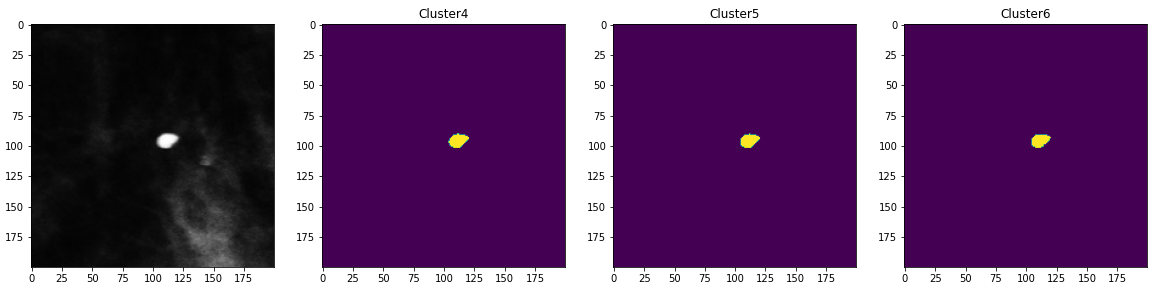
\includegraphics[scale=0.45]{images/segmented_fuzzy_c_means_tumor5.png}}
\centerline{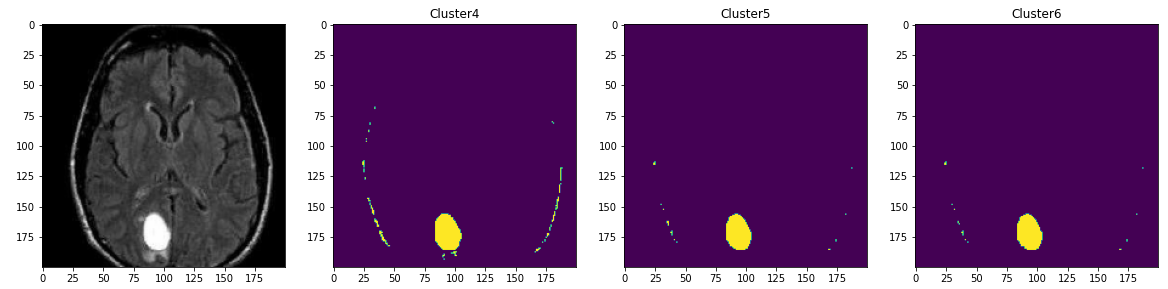
\includegraphics[scale=0.45]{images/segmented_fuzzy_c_means_tumor6.png}}
\end{figure}


\subsection{\fontencoding{OT2}\selectfont K-sredina}

K-sredina algoritam je iterativni algoritam koji poku\v{s}ava podeliti skup podataka u unapred zadat broj zasebnih podgrupa(klastera).

Sledi detaljan opis algoritma:

\begin{itemize}

\item Ulazni parametri: Podaci koje \v{z}elimo da klasterujemo (skup elemenata $x$ dimenizje $n$) i broj koji ozna\v{c}ava koliko klastera \v{z}elimo da dobijemo ($k$).
\item Izlazni paramteri: Matrica pripadnosti klasterima (dimenzije $n \times 2$ ) i matrica centroida klastera(dimenzije $k \times d$ gde je $d$ dimenzija svakog pojedina\v{c}nog elementa iz skupa $x$).

Koraci algoritma:

\begin{enumerate}

\item Navodimo \v{z}eljeni broj klastera.
\item Nasumi\v{c}no dodeljujemo vrednosti za centroide svih klastera u oznaci $c_j$. 
\item Ra\v{c}unanje centroida za sve klastere kao aritmeti\v{c}ke sredine svih elemenata u klasteru.
\item Za svaki podatak a\v{z}uriramo klaster kom on pripada tako da pripada klasteru \v{c}iji centroid mu je najbli\v{z}i.
\item Ponavljamo korake 2. i 3. dok centroidi ne ostanu isti u dve iteracije za redom.

\end{enumerate}

Mera kvaliteta klasterovanja je suma kvadratne gre\v{s}ke(eng. {\fontencoding{T1}\selectfont Sum of Squared Error}).

\subsubsection{\fontencoding{OT2}\selectfont Na\v{s}a implementacija algoritma k-sredina}

Re\v{s}enje problema segmentacije slika uz pomo\'{c} algoritma k-sredina smo implementirali u programskom jeziku Pajton (eng. {\fontencoding{T1}\selectfont Python}).\\
Pajton biblioteke kori\v{s}\'{c}ene u na\v{s}em re\v{s}enju su:
\begin{itemize}
\item $ numpy $
\item $ matplotlib.pyplot $
\item $ os $
\item $ cv2 $
\item $ time $
\item $ math $
\end{itemize} 
Algoritam je implementiran u funkciji $ k\_means() $. Ona kao argumente prima:
\begin{itemize}
\item $data$ - niz podataka(to je ustvari matrica koja je dimenzije $n \times d$);
\item $n$ - ceo broj koji ozna\v{c}ava broj podataka koje \v{z}elimo da klasterujemo;
\item $k$ - ceo broj koji ozna\v{c}ava broj klastera;
\item $d$ - ceo broj koji ozna\v{c}ava dimenziju pojedina\v{c}nog podatka iz skupa podataka koje \v{z}elimo da klasterujemo;
\item $max\_iter$ - ceo broj koji ozna\v{c}ava maksimalni broj iteracija zbog bezbednosti,
\end{itemize}
dok kao povratnu vrednost vra\'{c}a:
\begin{itemize} 
\item matricu $n \times 2$ u kojoj \'{c}e se uz element nalaziti oznaka klastera kom pripada;
\item matricu $k \times d$ u kojoj \'{c}e se \v{c}uvati centroidi svih klastera.
\end{itemize}
Dakle, kako je jedna slika predstavljena kao matrica piksela gde je svaki piksel dimenzije tri, nju parsiramo u niz, kori\v{s}\'{c}enjem funkcije  $ reshape() $ iz Pajton biblioteke $ numpy $, kako bismo je mogli, kao argument, proslediti na\v{s}oj funkciji. Nakon \v{s}to na\v{s}a funkcija kao povratnu vrednost vrati matricu pripadnosti podataka(u na\v{s}em slu\v{c}aju piksela dimenzije 3) klasterima svakom od piksela dodeljujemo vrednost centroida klastera kom pripada. Zatim niz piksela vra\'{c}amo u matricu polaznih dimenzija kori\v{s}\'{c}enjem funkcije  $ reshape() $ i posmatramo je kao sliku.

\subsubsection{\fontencoding{OT2}\selectfont Rezultati algoritma k-sredina}

Nakon opisanog postupka slike ispisujemo kori\v{s}\'{c}enjem funkcija $ subplot() $ i $ imshow() $ iz Pajton biblioteke $ cv2 $.\\
Slike koje je segmentovao na\v{s} algoritam k-sredina izgledaju ovako:

\end{itemize}

\newpage

\begin{figure}[h!]
\centerline{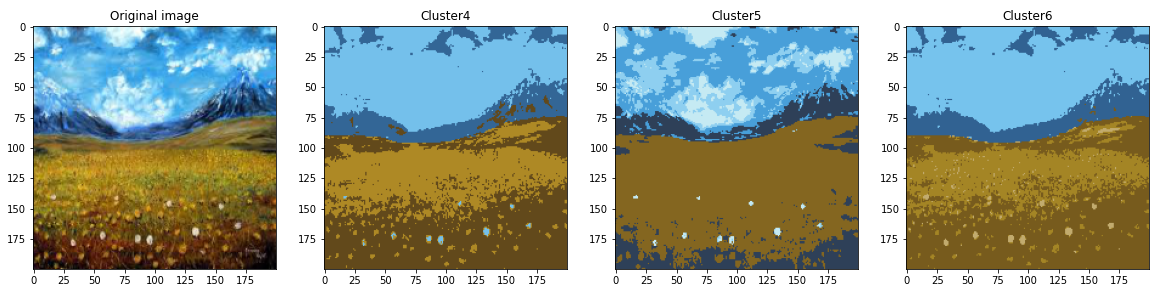
\includegraphics[scale=0.45]{images/segmented_k_means1.png}}
\centerline{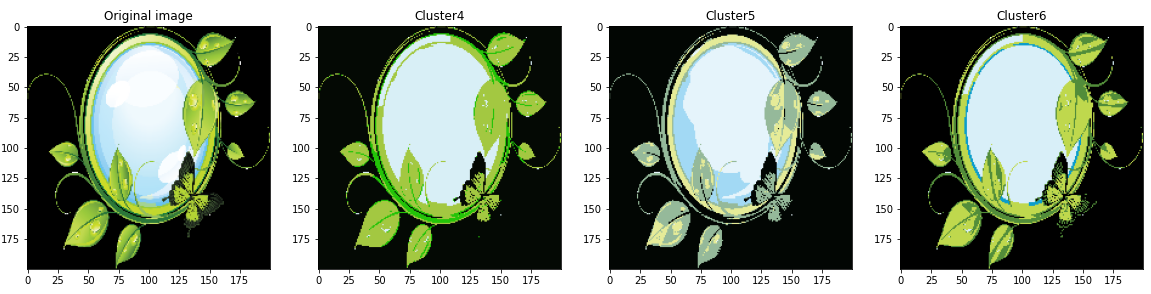
\includegraphics[scale=0.45]{images/segmented_k_means3.png}}
\centerline{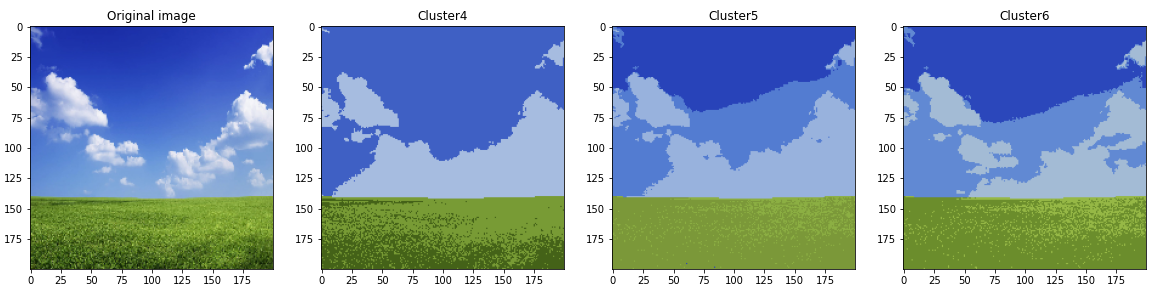
\includegraphics[scale=0.45]{images/segmented_k_means4.png}}
\centerline{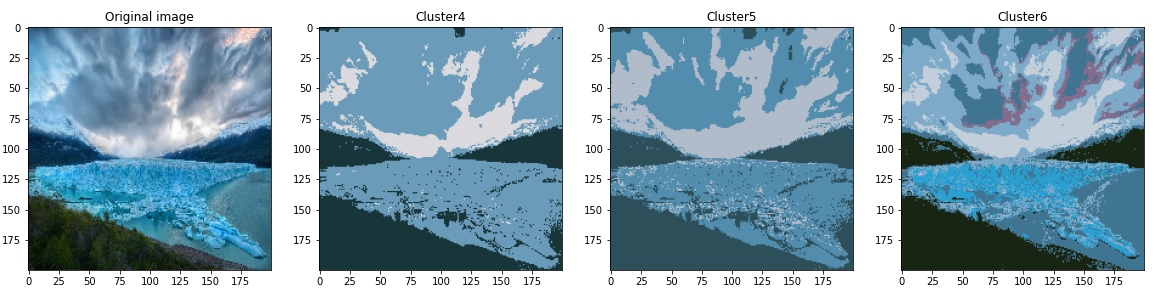
\includegraphics[scale=0.45]{images/segmented_k_means5.png}}
\end{figure}

\newpage

\begin{figure}[h!]
\centerline{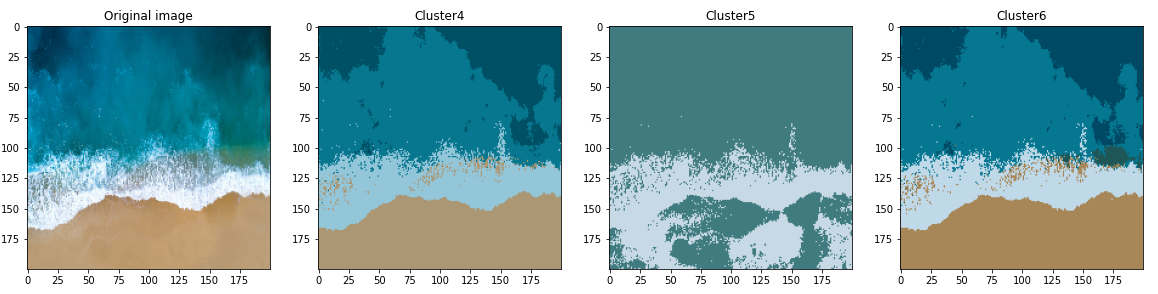
\includegraphics[scale=0.45]{images/segmented_k_means8.png}}
\centerline{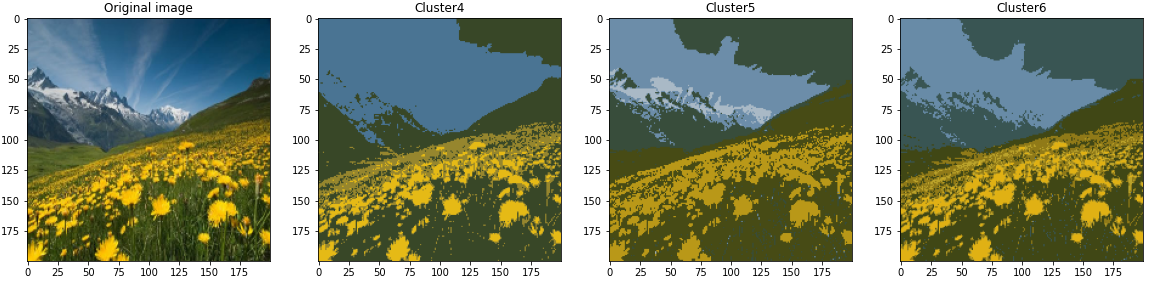
\includegraphics[scale=0.45]{images/segmented_k_means6.png}}
\centerline{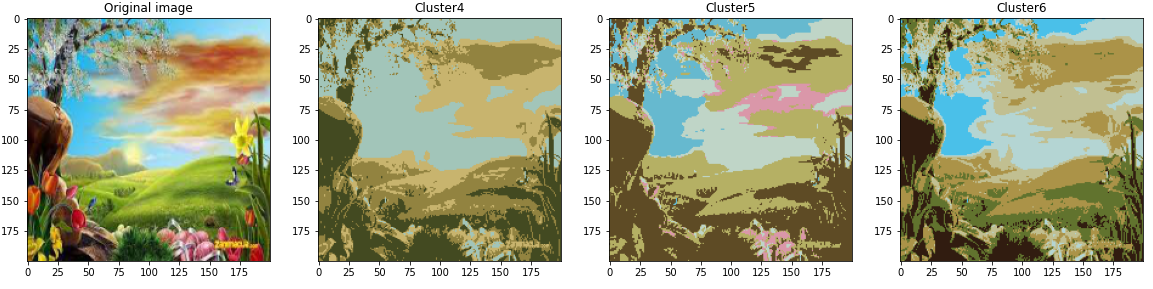
\includegraphics[scale=0.45]{images/segmented_k_means7.png}}
\centerline{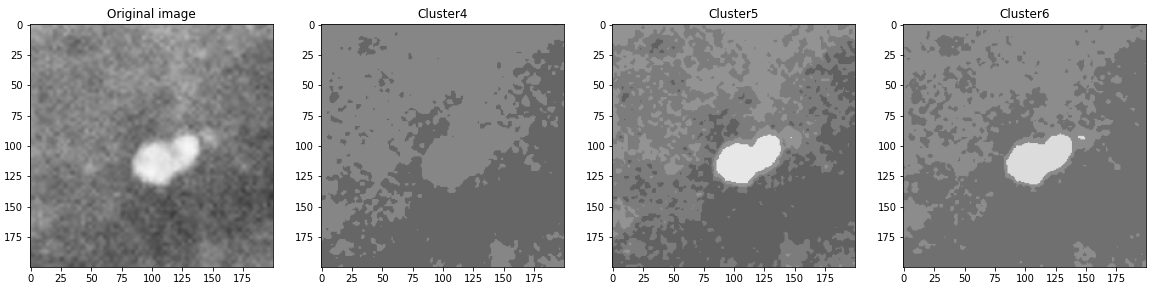
\includegraphics[scale=0.45]{images/segmented_k_means0.png}}
\end{figure}

\newpage

\begin{figure}[h!]
\centerline{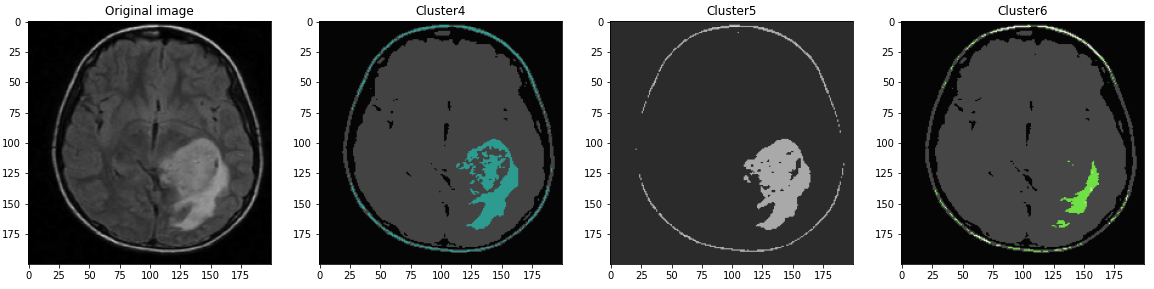
\includegraphics[scale=0.45]{images/segmented_k_means10.png}}
\centerline{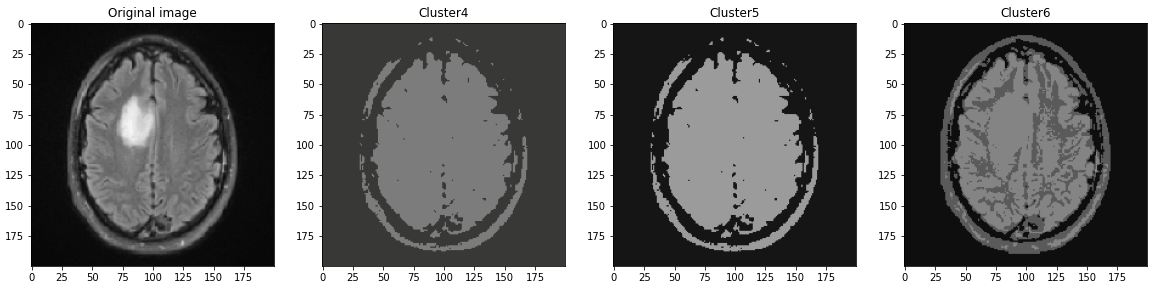
\includegraphics[scale=0.45]{images/segmented_k_means11.png}}
\centerline{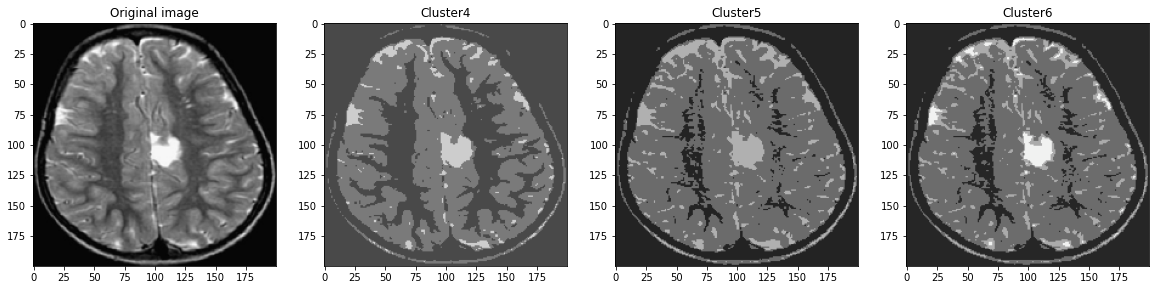
\includegraphics[scale=0.45]{images/segmented_k_means9.png}}
\centerline{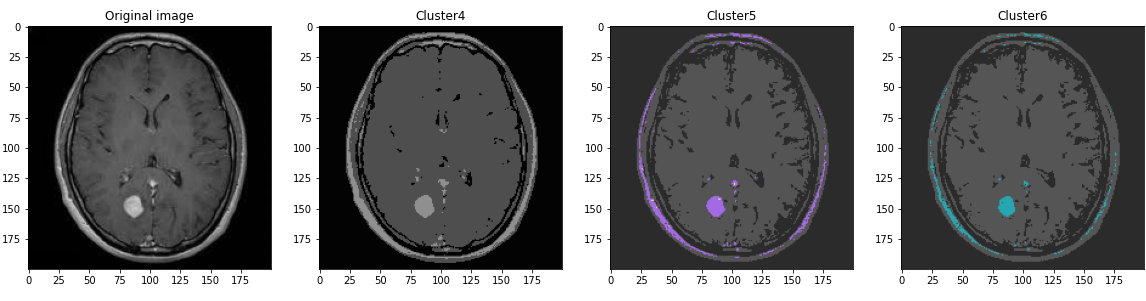
\includegraphics[scale=0.45]{images/segmented_k_means2.png}}
\end{figure}

\newpage

\begin{figure}[h!]
\centerline{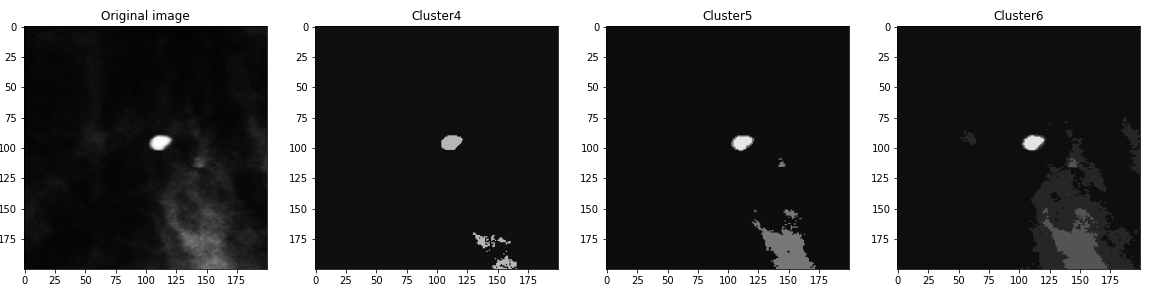
\includegraphics[scale=0.45]{images/segmented_k_means12.png}}
\centerline{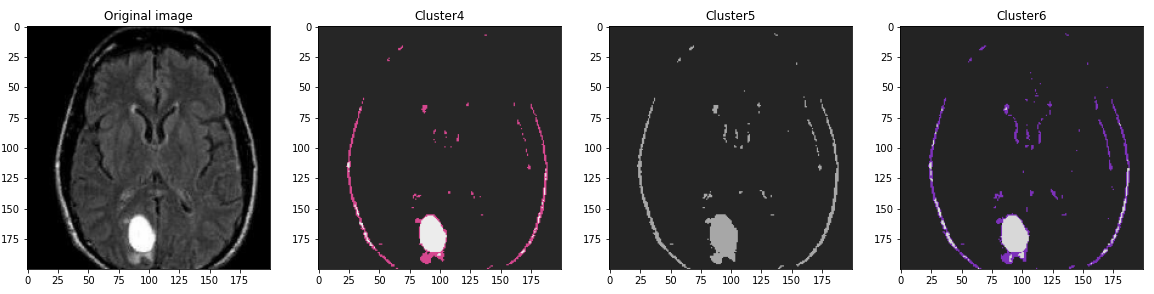
\includegraphics[scale=0.45]{images/segmented_k_means13.png}}

\end{figure}

U slu\v{c}aju rendgenskih snimaka mozga vrlo je bitno da se jasno segmentuje odre\dj eni detalj na slici, odnosno tumor ako on postoji, i zbog toga nakon gore opisanog postupka binarizujemo sliku kori\v{s}\'{c}enjem funkcije $ threshold() $ iz biblioteke $ cv2 $ i piksele predstavljamo jednom celobrojnom vredno\v{s}\'{c}u, odnosno predstavljamo sliku sa samo dve boje. Ovaj postupak je detaljno opisan u odeljku \ref{text:threshold}.\\


Nakon primene na\v{s}eg algoritma k-sredina, funkcije $ threshold() $ i parsiranja slike u matricu piksela koji su dimenzije jedan na rendgenske snimke tumora mozga na izlazu dobijamo slike segmentovane na slede\'{c}i na\v{c}in:

\newpage

\begin{figure}[h!]
\centerline{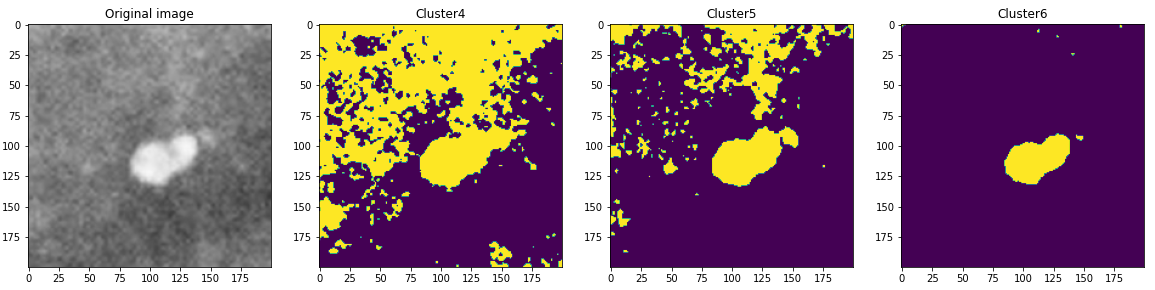
\includegraphics[scale=0.45]{images/segmented_k_means_tumor0.png}}
\centerline{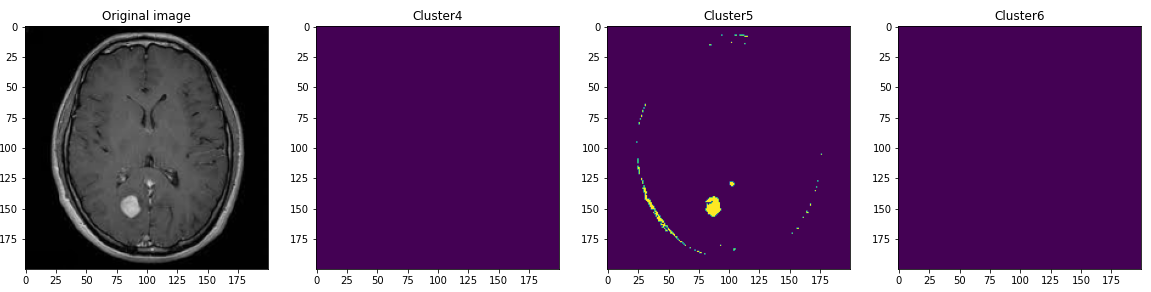
\includegraphics[scale=0.45]{images/segmented_k_means_tumor1.png}}
\centerline{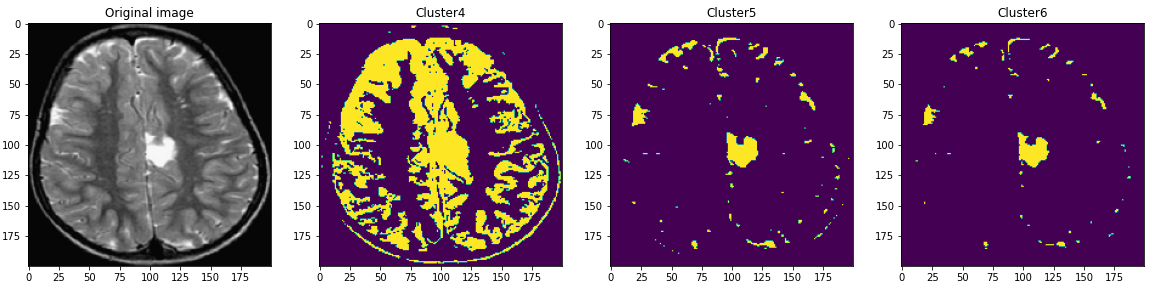
\includegraphics[scale=0.45]{images/segmented_k_means_tumor2.png}}
\centerline{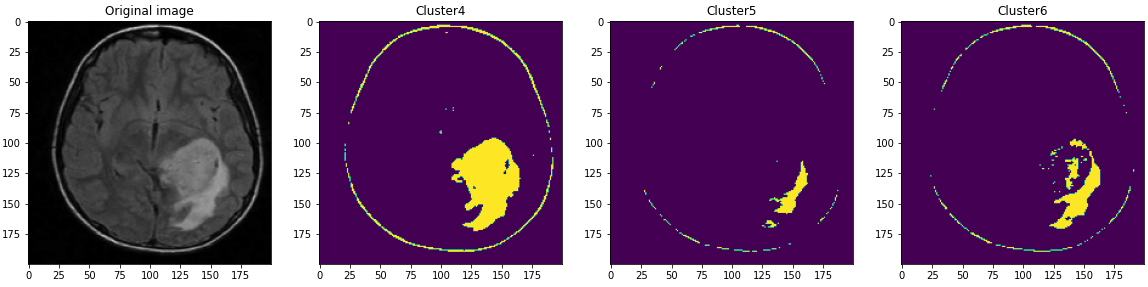
\includegraphics[scale=0.45]{images/segmented_k_means_tumor3.png}}
\end{figure}

\newpage

\begin{figure}[h!]
\centerline{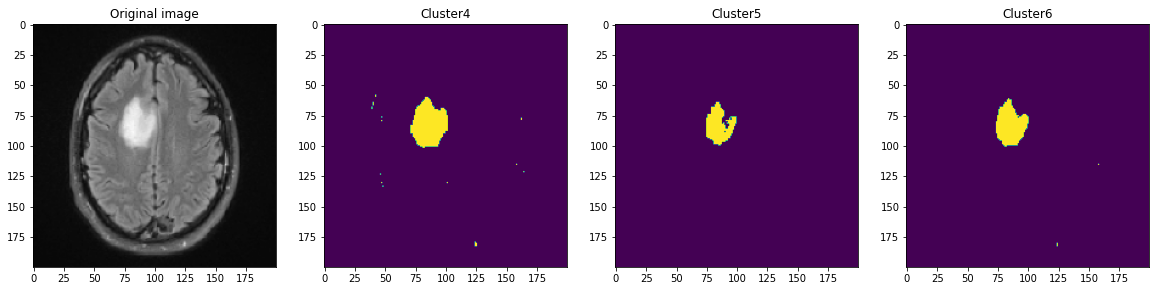
\includegraphics[scale=0.45]{images/segmented_k_means_tumor4.png}}
\centerline{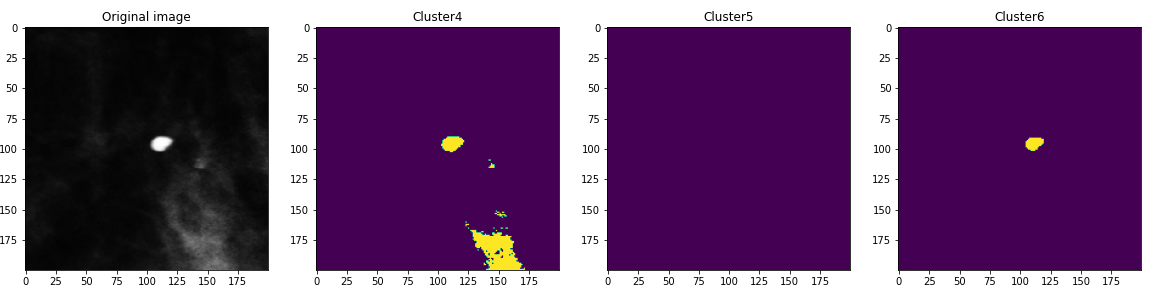
\includegraphics[scale=0.45]{images/segmented_k_means_tumor5.png}}
\centerline{\includegraphics[scale=0.45]{images/segmented_k_means_tumor6.png}}
\end{figure}


\subsection{\fontencoding{OT2}\selectfont Funkcija $ threshold() $ i predstavljanje piksela jednom vredno\v{s}\'{c}u}
\label{text:threshold}

Za rendgenske snimke tumora, nakon gore opisanog postupka (za oba algoritma), primenjena je funkcija $ threshold() $ iz Pajton biblioteke $ cv2 $ sa ciljem da tumor koji smo izdvojili bude obojen jednom bojom, a ostatak slike bude obojen potpuno druga\v{c}ijom bojom. Ovo radimo jer nam je bitno da tumor sa snimka bude jasno izdvojen. Funkcija $ threshold() $ kao argumente prima redom:
\begin{itemize}
\item sliku koju \v{z}elimo da obradimo (po\v{z}eljno je da slika bude sive boje, odnosno da svaki od piksela bude predstavljen sa tri iste vrednosti, kako bismo dobili smislene rezultate)
\item celobrojna vrednost koja predstavlja referentnu vrednost, koristi se za klasifikaciju vrednosti koje \v{c}ine piksele
\item celobrojna vrednost
\item parametar definisan na nivou biblioteke $ cv2 $ koji odre\dj uje kako \'{c}e raditi funkcija $ threshold() $
\end{itemize}

Za na\v{s}e potrebe koristi\'{c}emo $THRESH\_BINARY$ kao \v{c}etvrti argument funkcije i u tom slu\v{c}aju funkcija radi na slede\'{c}i na\v{c}in: Svaka od tri vrednosti svakog piksela se upore\dj uje sa referentnom vredno\v{s}\'{c}u, ukoliko je vrednost manja ili jednaka od referentne onda se ona zamenjuje sa nulom, a ako je ve\'{c}a onda se zamenjuje sa vredno\v{s}\'{c}u koja je zadata kao tre\'{c}i argument funkcije.\\

U na\v{s}em slu\v{c}aju kao referentnu vrednost uzimamo $ max\_value - 1 $ gde $ max\_value $ predstavlja najve\'{c}u vrednost u na\v{s}oj slici, dakle u tom slu\v{c}aju samo pikseli koji imaju ba\v{s} sve tri vrednosti $ maks\_value $ \'{c}e oti\'{c}i u tre\'{c}i argument dok \'{c}e svi ostali oti\'{c}i u nula. Drugim re\v{c}ima samo jedan klaster koji ima najve\'{c}u vrednost centroida \'{c}e biti izdvojen dok \'{c}e se svi ostali stopiti u jedan. Ovaj postupak nam je veoma koristan jer je tumor na rendgenskim snimcima svetliji od ostatka slike pa iz tog razloga \v{z}elimo da izdvojimo samo one piksele koji imaju najve\'{c}u vrednost jer \v{s}to je ve\'{c}a vrednost piksela to je on svetliji.\\

Kako je slika i na izlazu iz funkcije $ threshold() $ siva ukoliko je prosle\dj ena slika siva piksel mo\v{z}emo pretvoriti u samo jednu vrednost (jer su sivim slikama svi pikseli predstavljeni sa tri iste vrednosti). Slike na izlazu su ljubi\v{c}asto \v{z}ute jer pikseli sada nisu predstavljeni sa tri vrednosti (kojima bismo mi odre\dj ivali boju) ve\'{c} sa jednom i u tom slu\v{c}aju se koristi podrazumevana mapa boja(ukoliko imamo dve razli\v{c}ite vrednosti koje odre\dj uju piksele na nivou cele slike manja \'{c}e biti predstavljena ljubi\v{c}astom, a ve\'{c}a \v{z}utom bojom).


\subsection{\fontencoding{OT2}\selectfont Pore\dj enje rezultata}

Pore\dj enjem rezultata koje vra\'{c}aju algoritmi k-sredina i fazi c-sredina mo\v{z}emo videti da su slike primetno bolje segmentovane algoritmom fazi c-sredina. Njegova slo\v{z}enost je ve\'{c}a od slo\v{z}enosti algoritma k-sredina pa sam proces segmentacije traje ne\v{s}to du\v{z}e. Tako\dj e prednost algoritma fazi c-sredina je to \v{s}to se u praksi pokazalo da daje skoro potpuno iste rezultate za isti broj klastera na istim slikama, dok kod algoritma k-sredina to nije slu\v{c}aj. Razlog tome je \v{s}to algoritam k-sredina veoma zavisi od pseudo-slu\v{c}ajno zadatih po\v{c}etnih vrednosti centroida klastera.

\section{\fontencoding{OT2}\selectfont Zaklju\v{c}ak}

Klasterovanje je jedan od najkori\v{s}\'{c}enijih na\v{c}ina za segmentaciju slika. Ogromna prednost fazi klasterovanja u odnosu na ostale tehnike segmentacije slika je to \v{s}to je vrlo otporan na nepravilne granice. Tokom rada koristili smo vi\v{s}e razli\v{c}itih slika koje smo segmentovali uz isprobavanje razli\v{c}itih vrednosti odre\dj enih parametara i razli\v{c}itog broja klastera. U ve\'{c}ini slu\v{c}ajeva, kod fazi c-sredina algoritma, za izdvajanje tumora sa rengenskih snimaka najbolje se pokazalo kori\v{s}\'{c}enje 5 klastera, a za segmentaciju slika u boji broj klastera koji je najbolje koristiti zavisi od toga koliko detaljna segmentacija nam je potrebna, u obe situacije najbolje se pokazalo da je parametar fazi formule ($p$) jednak 2. Kod k-sredina algoritma se ne mo\v{z}e jednostavno utvrditi za koji broj klastera dobijamo najbolje rezultate s obzirom na to da smo u nekim situacijama pri radu sa eksperimentalnim podacima dobijali najbolju segmentaciju za jedan broj klastera, a onda kada bismo opet pokrenuli algoritam najbolja segmentacija bi se dobila za drugi broj klastera razlog tome je zavisnost algoritma k-sredina od po\v{c}etnih pseudo-slu\v{c}ajnih vrednosti centroida. Kod oba algoritma vrednosti centroida smo poredili na dve decimale jer u tom slu\v{c}aju dobijamo pribli\v{z}no jednako dobre rezultate kao da smo poredili na vi\v{s}e decimala, ali mnogo ranije se zaustavljamo. Segmentacija slika uz pomo\'{c} algoritama fazi klasterovanja je svoju primenu izme\dj u ostalog na\v{s}la u medicini gde je veoma bitna preciznost rezultata. Naravno, fazi klasterovanje ima \v{s}irok spektar primene pored segmentacije slika u raznim drugim oblastima neke od njih su ekonomija, ve\v{s}ta\v{c}ka inteligencija i druge.

\newpage
\section{\fontencoding{OT2}\selectfont Literatura}

\fontencoding{T1}\selectfont
\begin{itemize}
\item M.S. YANG - A Survey of Fuzzy Clustering, October 1993.
\item XL Xie, G Beni - A validity measure for fuzzy clustering, 1991.
\item Donald E. Gustafson, William C. Kessel - Fuzzy clustering with a fuzzy covariance matrix, 1979.
\item Imad Dabbura - K-means Clustering: Algorithm, Applications, Evaluation Methods, and Drawbacks, September 2018
\fontencoding{OT2}\selectfont
\item Mirjana Maljkovi\'{c} - Skalabilni klaster algoritmi, 2008.
\item Nenad Miti\'{c} - Predavanje o klaster analizi na Matemati\v{c}kom fakultetu, 2020.
\end{itemize}


\end{document}